\section{Behaviour of the NTK}
\label{sec:NTKPheno}

\ac{General comments: the paging of the figuers is all messed up, but I will fix it once we
know what we want to keep (and discard).}
The NTK, introduced in Sec.~\ref{sec:GradFlow}, provides a powerful framework
for understanding neural network dynamics during training. Originally developed
by Jacot et al.~\cite{jacot2018neural} to analyze infinite-width feed-forward
networks, the NTK theory has since been extended to diverse architectures
including convolutional networks~\cite{arora2019exact} and recurrent
networks~\cite{alemohammad2021recurrent}. This theoretical framework has proven
invaluable for characterizing learning dynamics and generalization properties
across various network designs.

From Eq.~\eqref{eq:FlowEquationNoIndices}, we observe that the NTK encodes the
dependence on the architecture of the network and governs its training dynamics.
The analysis of the NTK properties is thus crucial for understanding the network
behaviour during training. We first show the properties of the NTK at
initialisation, before moving to the training phase, where we provide a detailed
study of the NTK in the context of the NNPDF methodology. To this end, we
performed a fit of $T_3$ using the NNPDF methodology with the dataset described
in Sec.~???. We initialized an ensemble of $N_{\rm Rep} = 100$ replicas with
identical architecture, training each independently using gradient descent (GD)
optimization. As our focus here is on NTK properties rather than physical
predictions, we employ synthetic data with controlled noise characteristics,
namely L0, L1, and L2 data generations. Throughout training, we track the
evolution of the NTK to understand how the network's effective dynamics change
as it learns the target function.

% ===================================
\begin{figure}[t!]
  \centering
  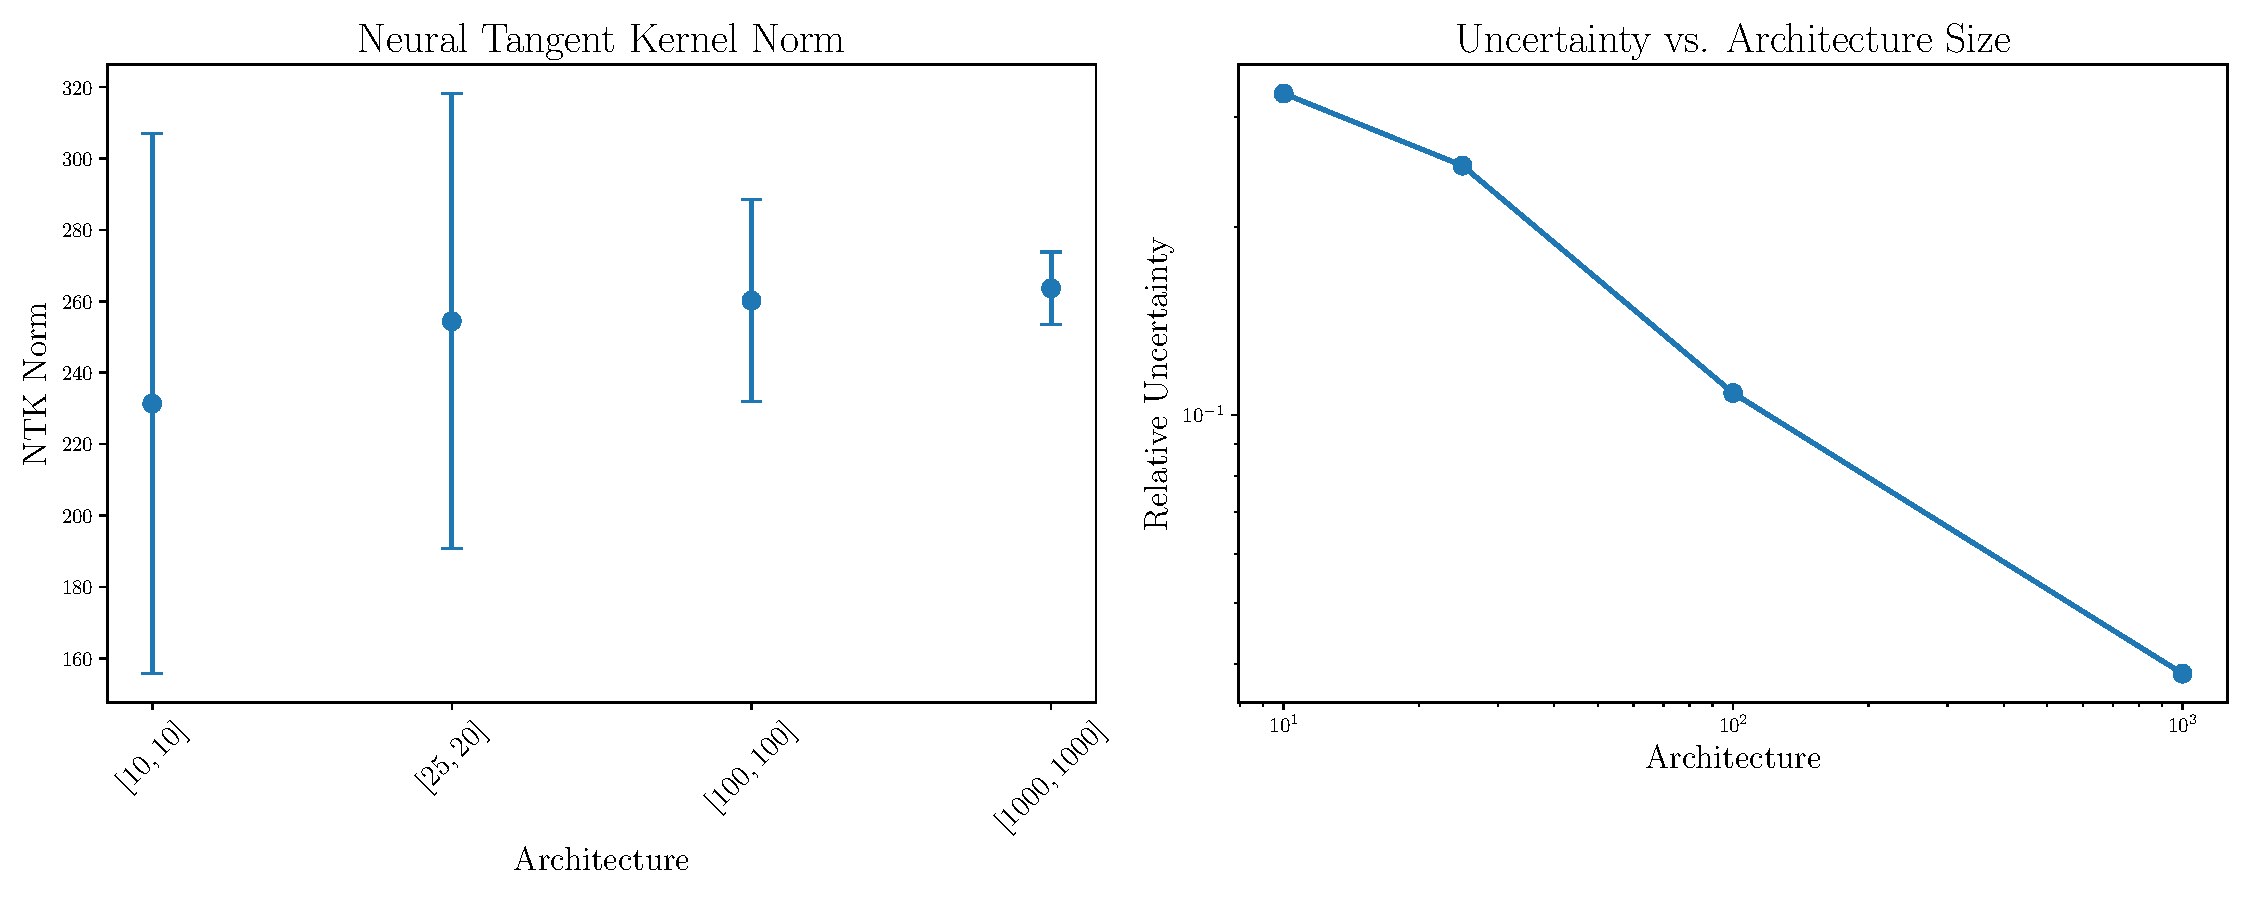
\includegraphics[width=0.90\textwidth]{../plots/ntk_initialization_with_uncertainty.pdf}
  \caption{Frobenius norm of the NTK at initialisation, $\lVert \Theta_0
  \rVert$, in function of the width of the network. On the left, central values
  and uncertainty bands are obtained as mean and one-sigma deviation of the
  ensemble of networks (left). The relative uncertainty is also shown (right)}
  \label{fig:NTKInit}
\end{figure}
% ===================================

% ===================================
\begin{figure}[t!]
  \centering
  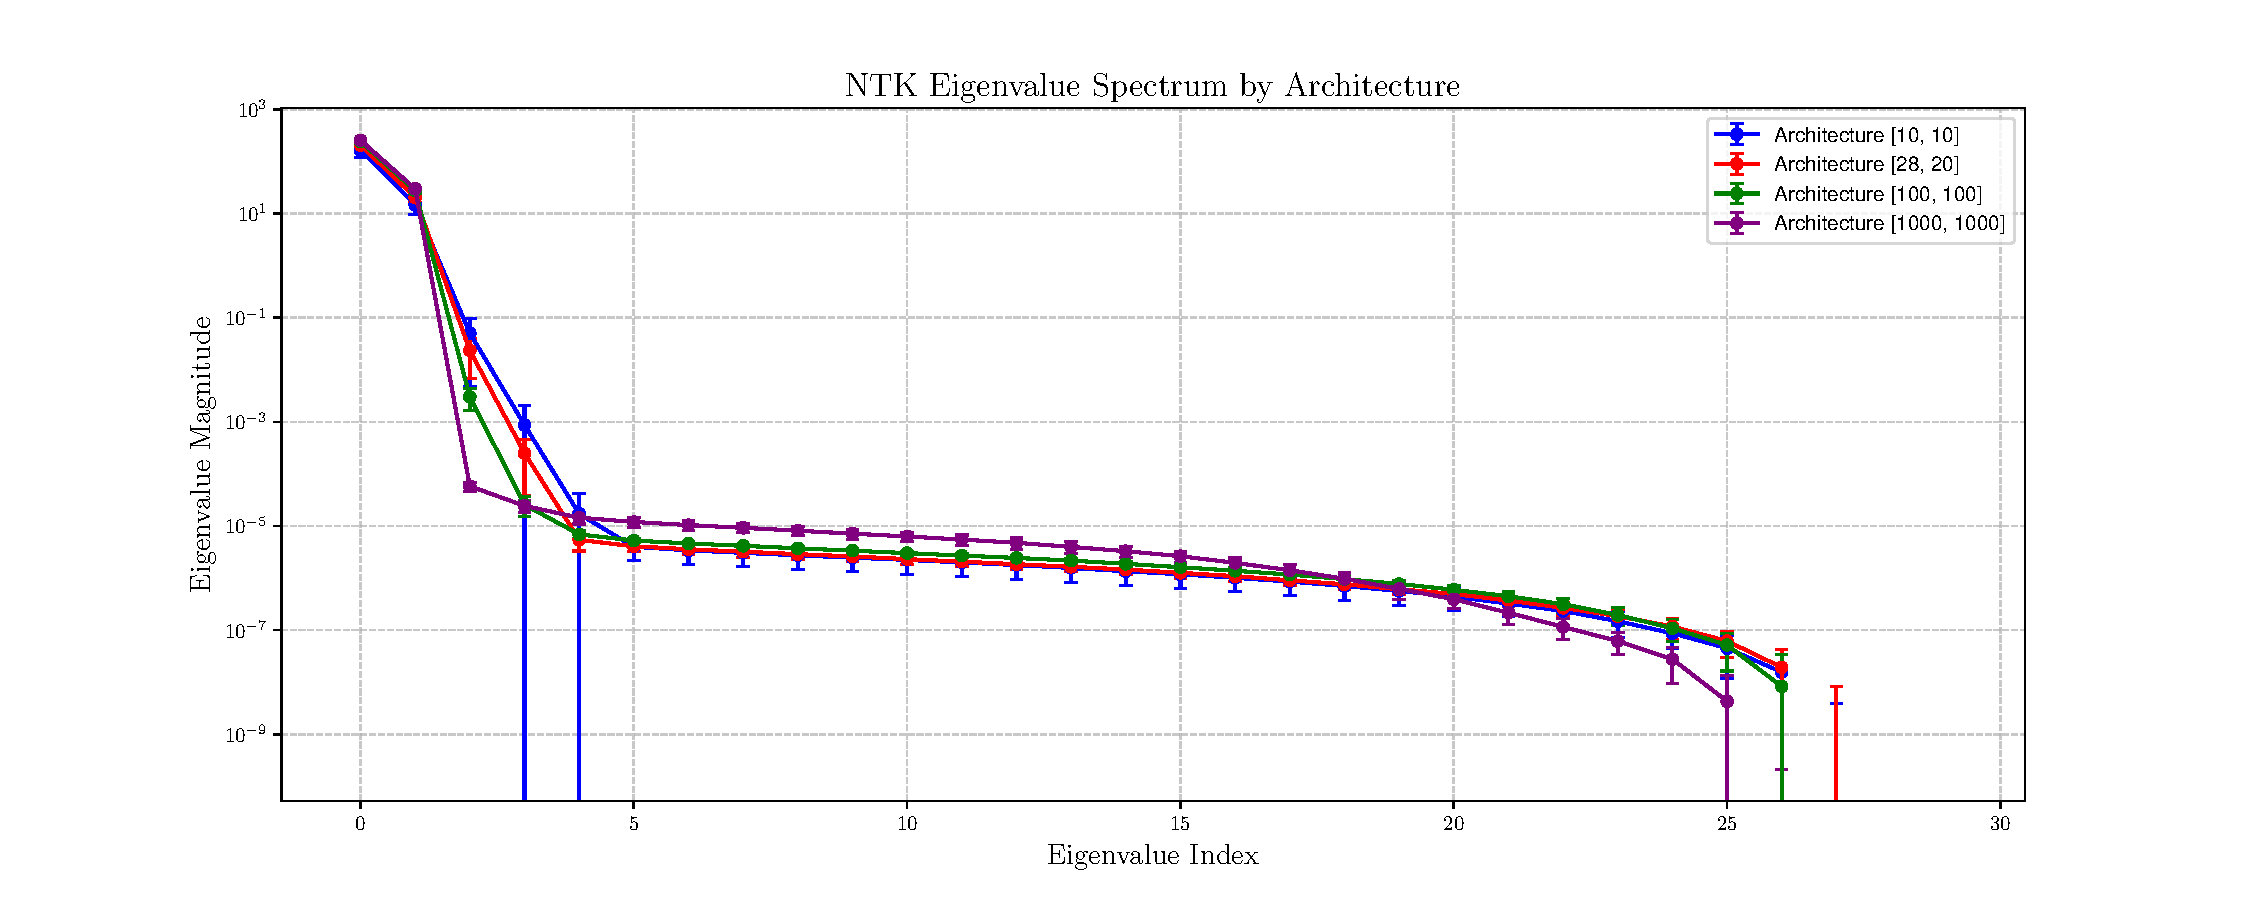
\includegraphics[width=0.90\textwidth]{plots/ntk_eigenvalue_spectrum.pdf}
  \caption{Spectrum of the NTK for the first three architectures displayed in
  Fig.~\ref{fig:NTKInit}. \ac{I'm thinking of removing uncertainty bands.}}
  \label{fig:NTKSpectrum}
\end{figure}
% ===================================
We first discuss the properties of the NTK at initialisation, that is when the
network is not blind to data. We remind that, at this stage, the NTK depends on
the $x$-grid of input and on the architecture. It is argued in the literature
that, in the large-width limit, the variance of the NTK tends to zero with the
size of the architecture (see, \textit{e.g.}, \cite{Roberts:2021fes}). In order
to assess this property of the NTK, we computed the Frobenius norm of the NTK
over an ensemble of networks for different architectures. For each architecture,
we took mean value and standard deviation as statistical estimators of the
ensemble. The result is displayed in Fig.~\ref{fig:NTKInit}. From this figure,
we can confirm that the variance of the NTK becomes smaller with the size of the
network. Note that, in addition to the scaling $\mathcal{O}(1/n)$ theoretically
predicted in the large networks, the uncertainty bands include bootstrap errors
due to the finite size of the ensemble. \ac{I can say something more here.}

Another feature of the NTK is shown in Fig.~\ref{fig:NTKSpectrum}, where the
spectrum of the NTK is shown for four different architectures. As debated in the
literature, the spectrum of the NTK is heavily hierarchical, and only few
eigenvalues are actually non-zero\footnote{Note that, due to the large
difference in magnitude of the eigenvalues, the relative precision of the
machine introduces noise noise in the decomposition, so that small eigenvalues
should be effectively considered zero. We will discuss the cut-off tolerance
later, when will discuss the training process in more details.}. This means that
only a small subset of active directions can inform the network during training,
as it will be discussed later. Note that, at least at initialisation, these
observations do not depend on the architecture.

% ===================================
\begin{figure}[h!]
  \centering
  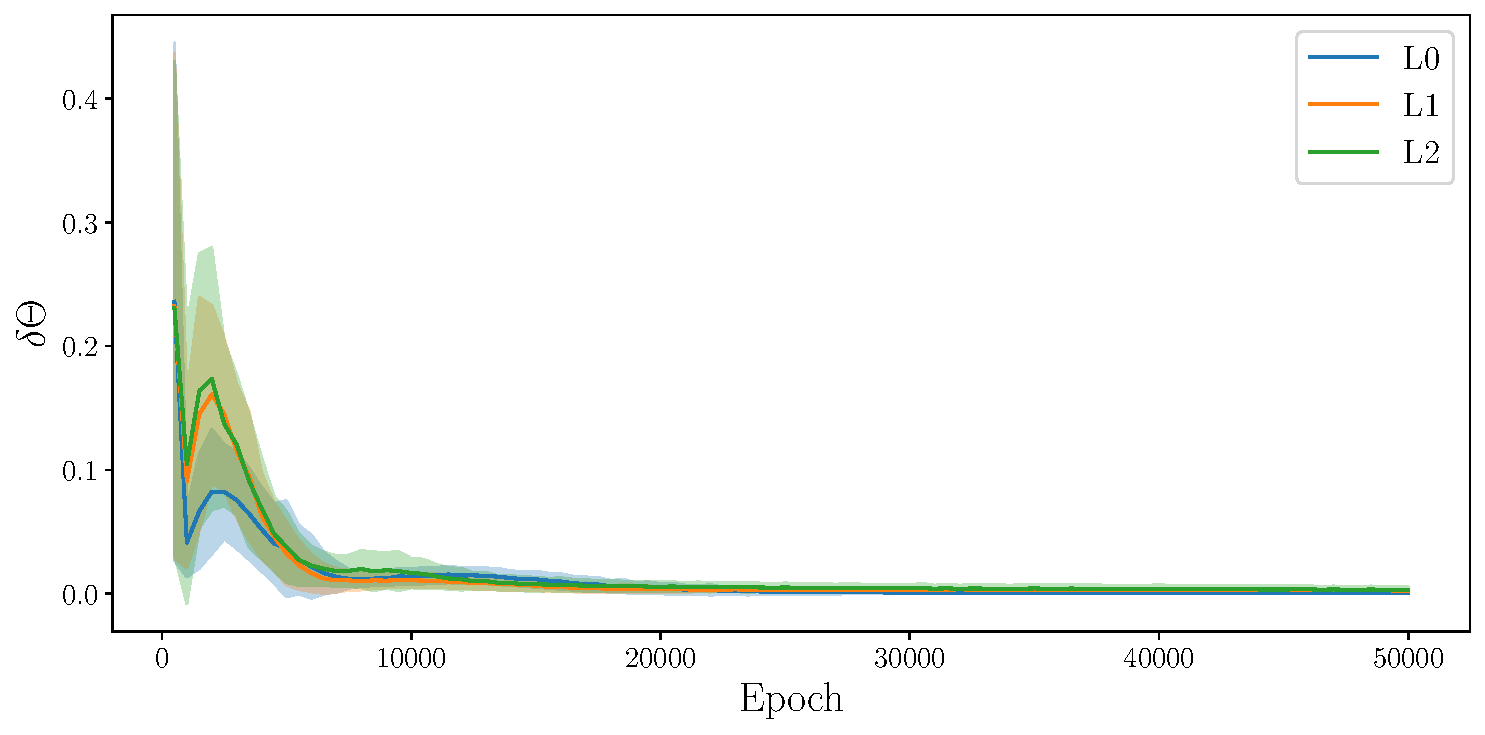
\includegraphics[width=0.6\textwidth]{../plots/delta_ntk.pdf}
  \caption{Relative variation of the NTK during training for L0, L1, and L2 data. Error
  bands correspond to one-sigma uncertainties over the ensemble of networks.}
  \label{fig:NTKTime}
\end{figure}
% ===================================
Having established the properties of the NTK at initialisation, we now discuss
its behaviour during training. In the machine learning literature, it is argued
that the NTK remains constant during training provided that the width of the
network is large enough. Here we show that this is not the case, at least for
the NNPDF methodology. In Fig.~\ref{fig:NTKTime}, we show the relative variation
of the Frobenius norm of the NTK
\begin{equation}
\delta \Theta_t = \frac{\lVert \Theta_{t+1} - \Theta_t \rVert}{\lVert \Theta_t \rVert} \;,
\label{eq:DeltaNTK}
\end{equation}
during training for three different datasets, L0, L1,
and L2. We observe that the NTK does not remain constant during training, but
rather it tends to change with time. In the figure, we can identify two
different phases. The first one covers the initial part of the training. From
Fig.~\ref{fig:NTKTime}, we see that the is rather sensitive to the evolution, in
strong contrast with the observations argued in the machine learning literature.
Note also that this initial peak is more pronounced for L2 data. This is
consistent with the fact that the NTK (\textit{i.e.}, the architecture) needs to
accommodate the noise in the data, thus leading to a larger variation of the
NTK. On the other hand, after this initial phase, the NTK tends to stabilize. We
will refer to this second phase as the \textit{lazy training}, in keeping with
the terminology adopted in the literature. We conclude that, in this phase, the
NTK does not change significantly. As a consequence, this suggests that the
theory of the infinite-width networks during training can be applied only after
the initial phase, when the NTK has stabilized, as discussed later in this
article.

% ===================================
\begin{figure}[h!]
  \centering
  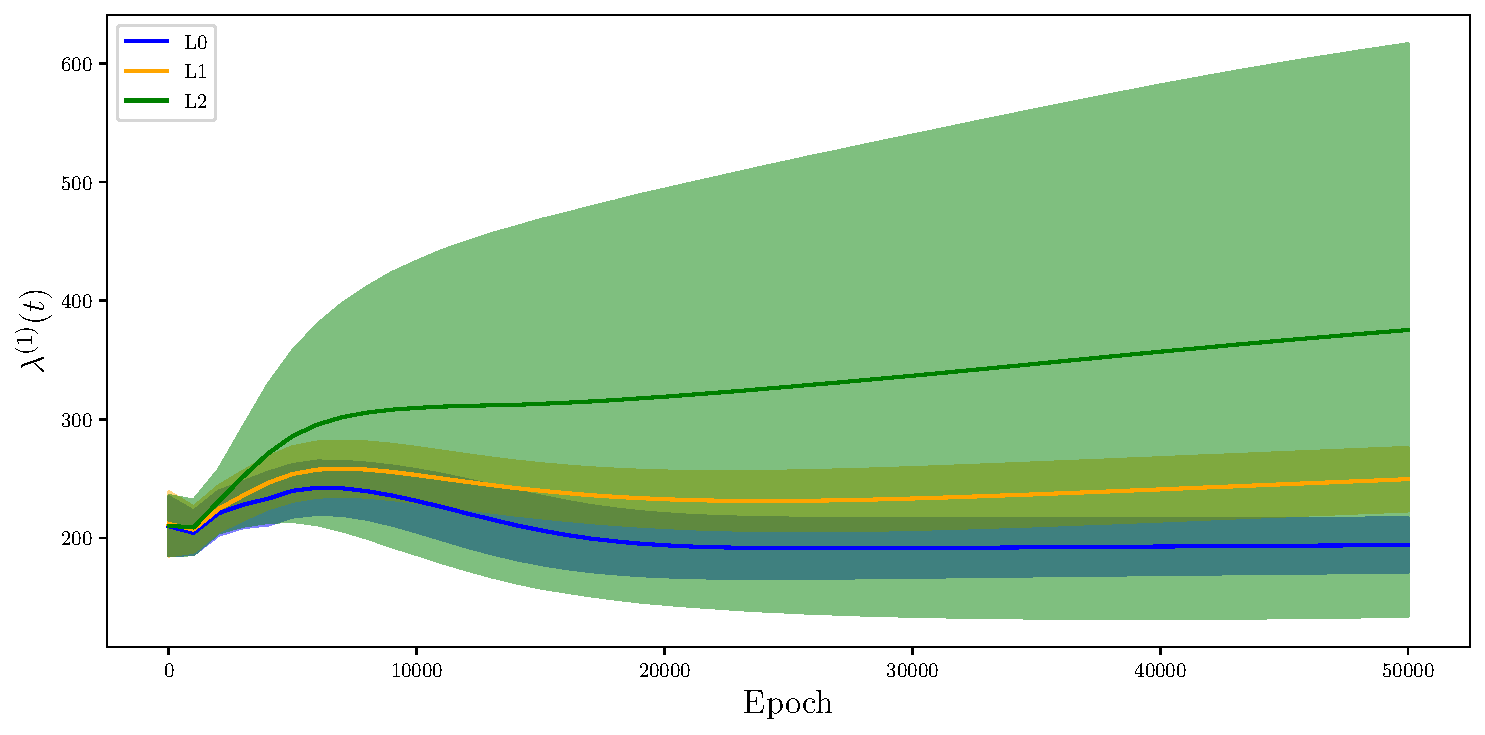
\includegraphics[width=0.48\textwidth]{../plots/eigval_1.pdf}
  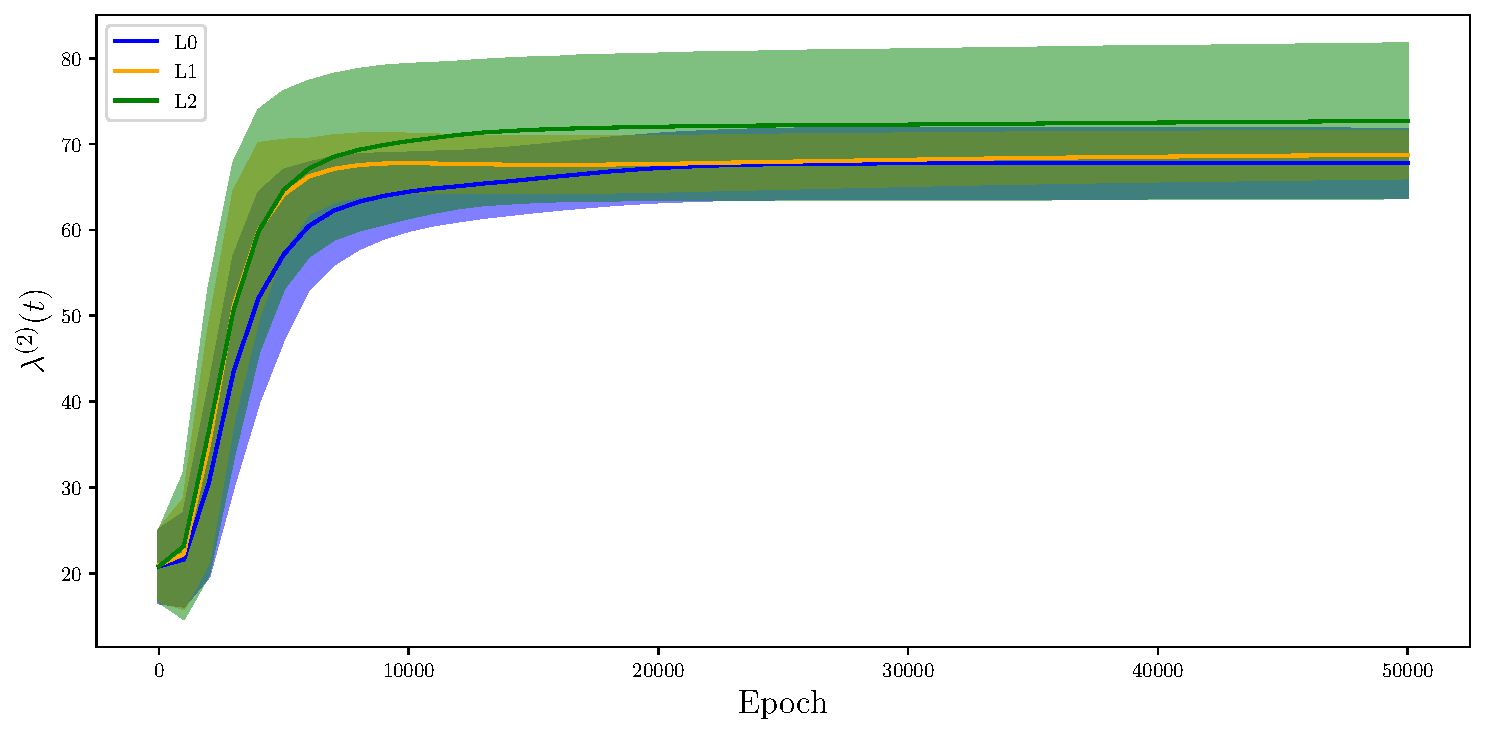
\includegraphics[width=0.48\textwidth]{../plots/eigval_2.pdf}
  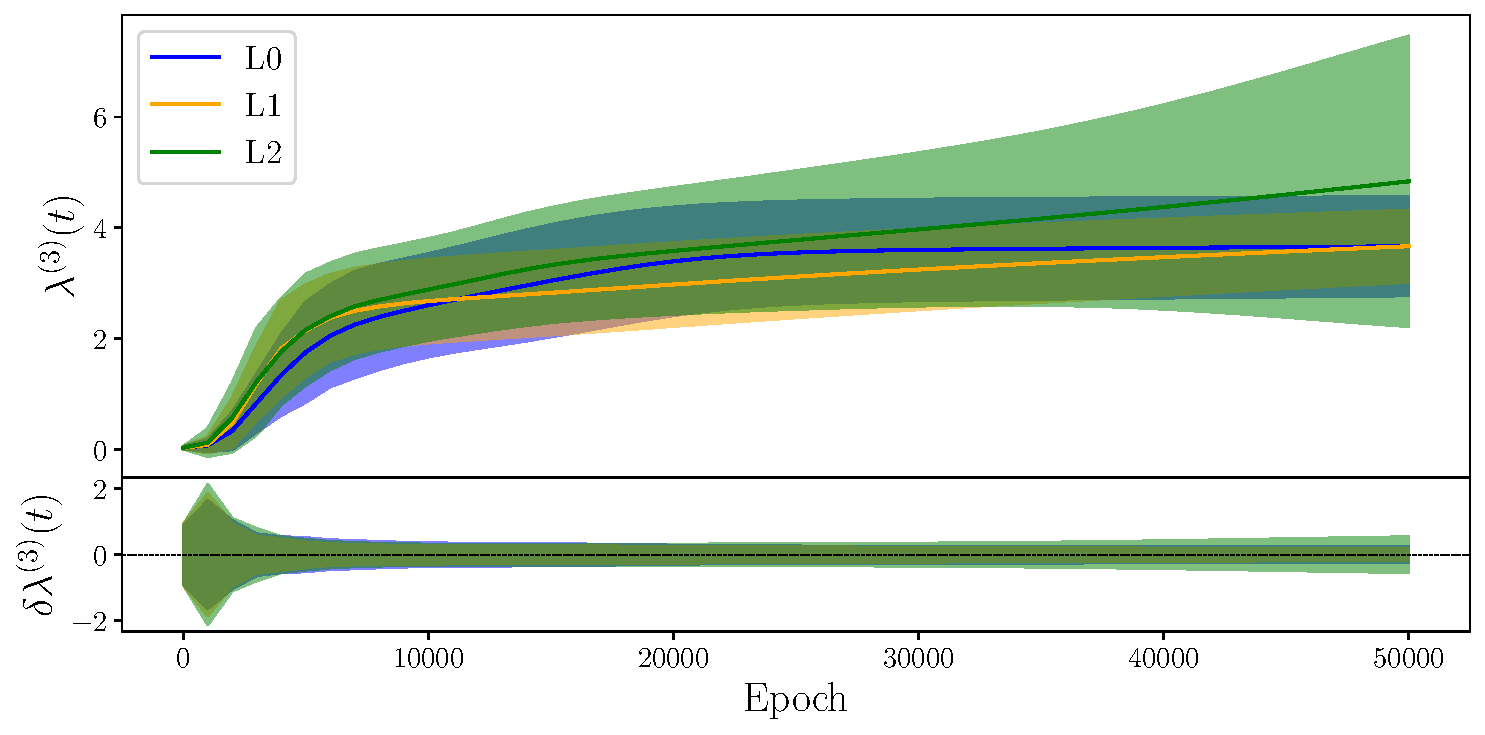
\includegraphics[width=0.48\textwidth]{../plots/eigval_3.pdf}
  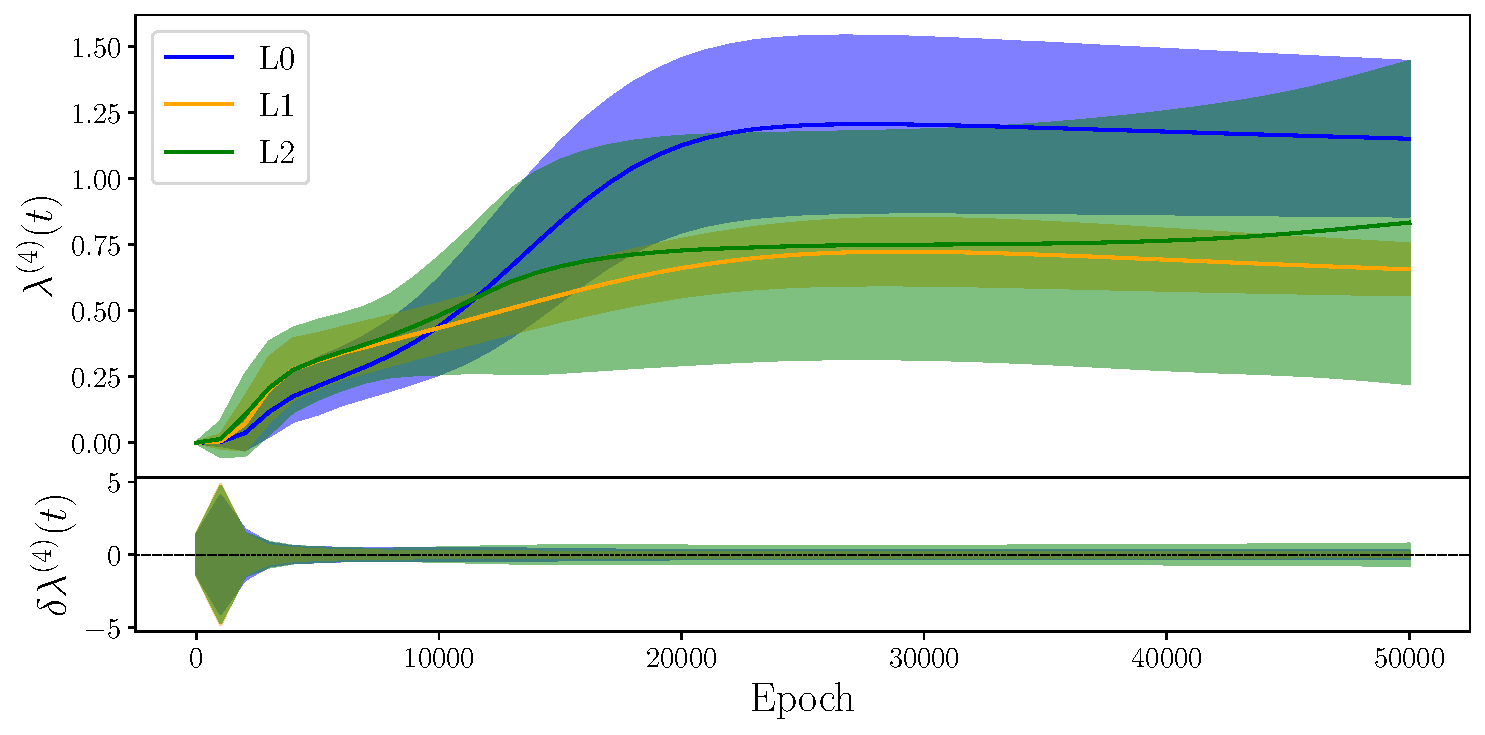
\includegraphics[width=0.48\textwidth]{../plots/eigval_4.pdf}
  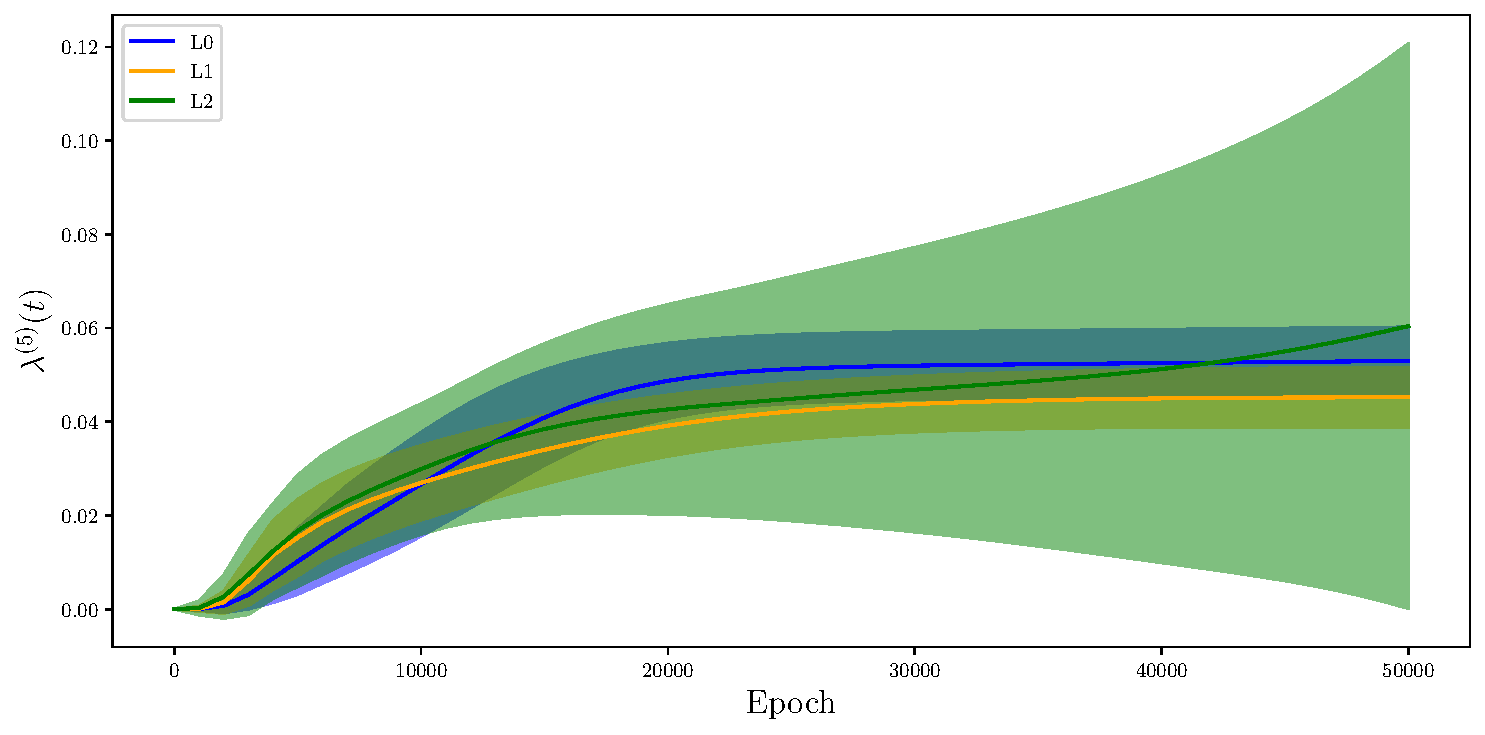
\includegraphics[width=0.48\textwidth]{../plots/eigval_5.pdf}
  \vspace{0.5cm}
  \caption{The first five eigenvalues of the NTK for L0, L1, and L2 data. Error
  bands correspond to one-sigma uncertainties over the ensemble of networks.}
  \label{fig:EigvalsComparison}
\end{figure}
% ===================================
One may ask how the eigenvalues of the NTK contribute to the variation of the
NTK. In Fig.~\ref{fig:EigvalsComparison}, the first five eigenvalues of the NTK
are displayed for L0, L1, and L2 data. We can make a few observations upon
inspecting these plots. First, we notice that the way in which data is generated
has an impact on the eigenvalues of the NTK. In general, the uncertainty bands
for L2 data are larger than those for L1 and L0 data, indicating that the NTK is
more sensitive to the noise in the data. This is consistent with the observation
made in Fig.~\ref{fig:NTKTime}. Second, we observe that the initial hierarchy of
the eigenvalues, Fig.~\ref{fig:NTKSpectrum}, is not preserved during training.
While the first eigenvalue remains dominant, the other eigenvalues grow with
time. This fact, combined with the analysis of Eq.~\eqref{eq:FlowSolution}
\ac{(this reference will be likely changed)}, suggests that more ``physical''
features become learnable during training. Most importantly, being these values
non-zero, they can be learned in a finite time and not require
$T\rightarrow\infty$ to be learned, which is unpractical.

% ===================================
\begin{figure}[h!]
  \centering
  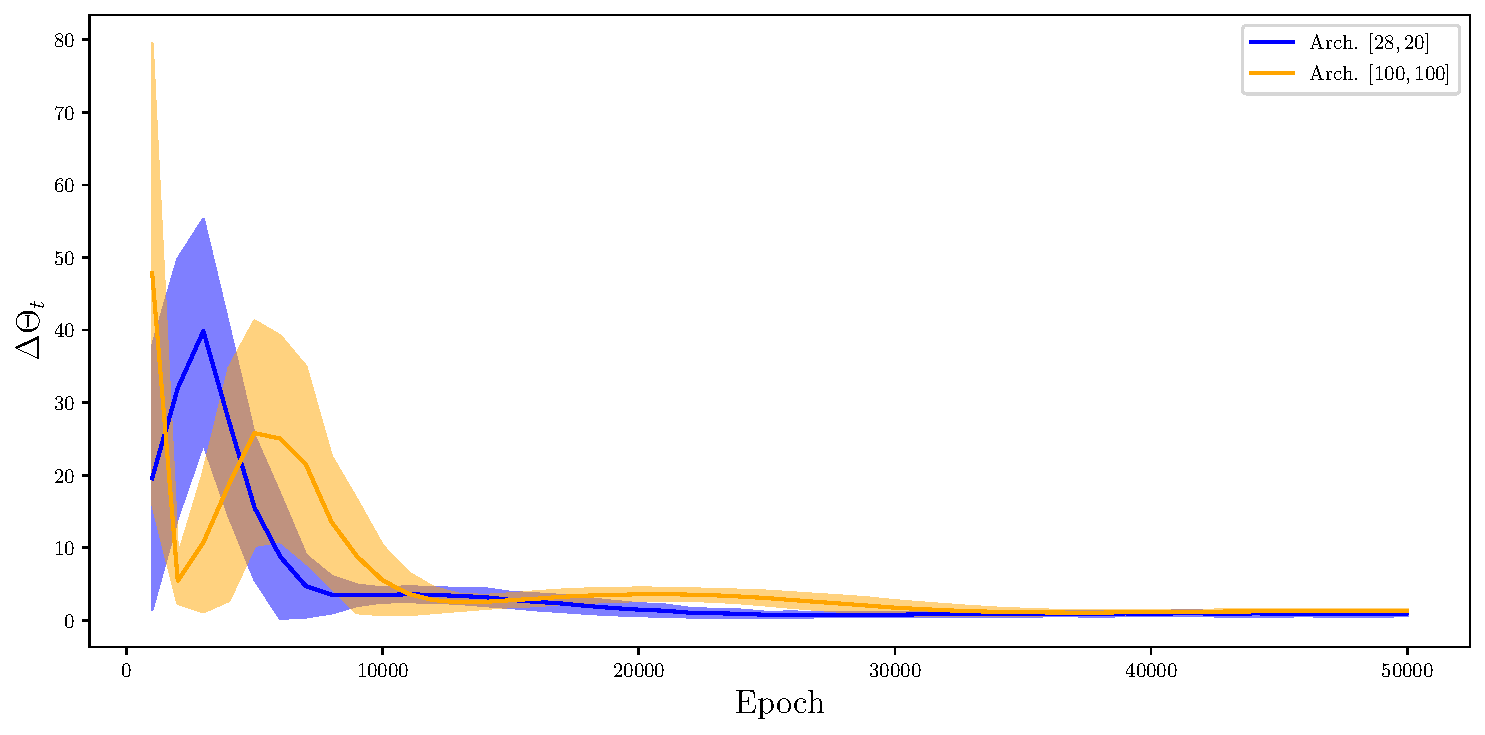
\includegraphics[width=0.6\textwidth]{../plots/delta_ntk_arch_L1.pdf}
  \caption{Comparison of the variation of the NTK during training for two
  different architectures with sizes $[28,20]$ and $[100,100]$ respectively. In
  both cases, L1 data are used. Error bands correspond to one-sigma
  uncertainties over the ensemble of networks.}
  \label{fig:NTKTimeDiffArch}
\end{figure}
% ===================================

% ===================================
\begin{figure}[h!]
  \centering
  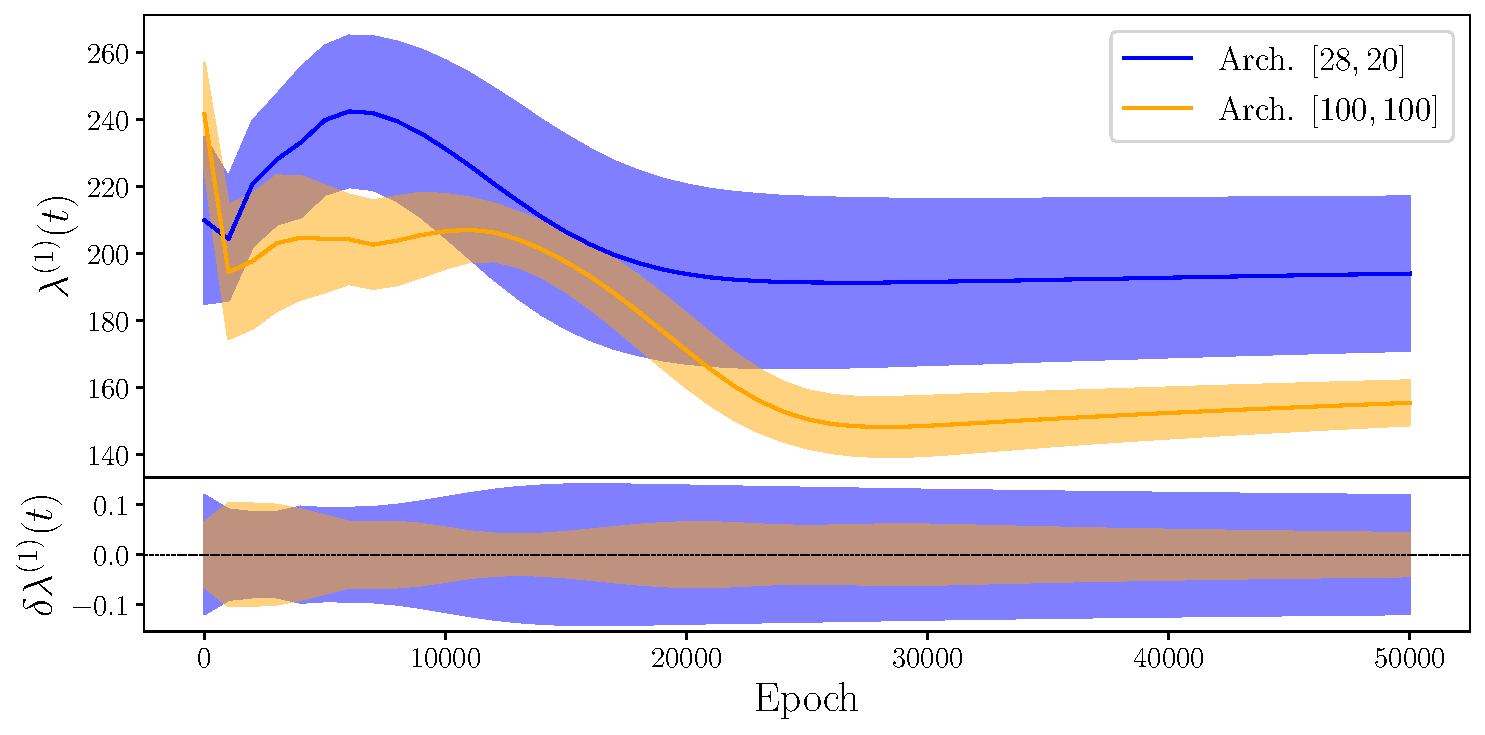
\includegraphics[width=0.48\textwidth]{../plots/eigval_1_arch_L0.pdf}
  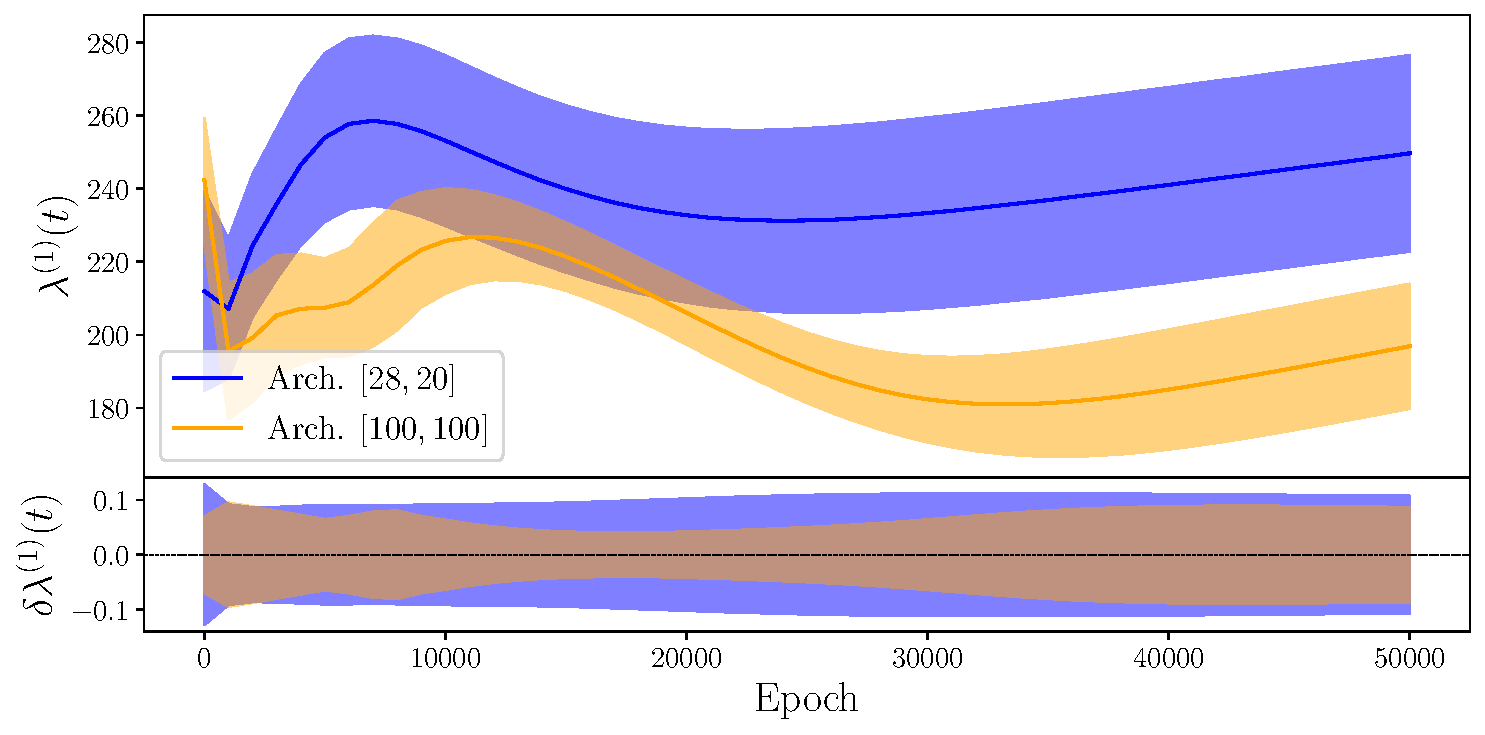
\includegraphics[width=0.48\textwidth]{../plots/eigval_1_arch_L1.pdf}
  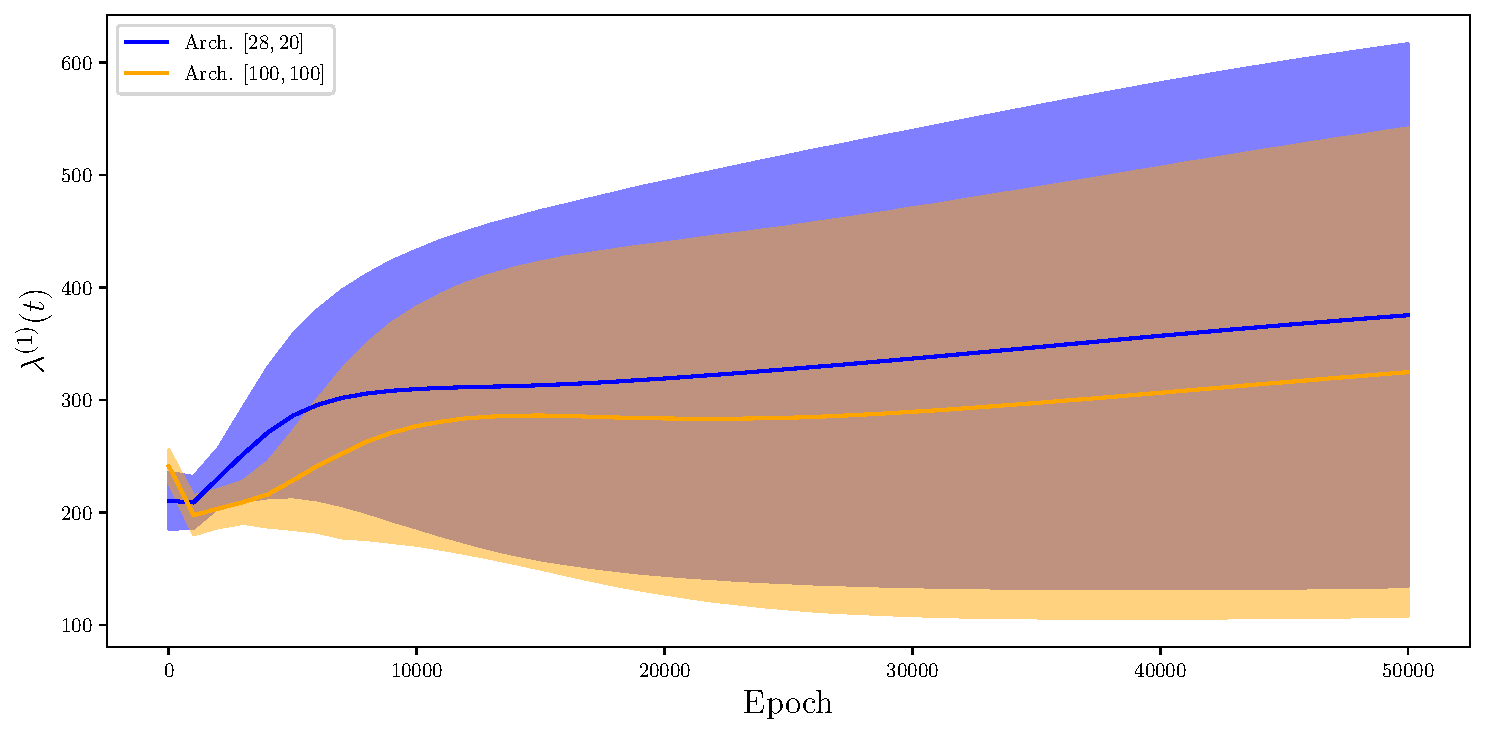
\includegraphics[width=0.48\textwidth]{../plots/eigval_1_arch_L2.pdf}
  \vspace{0.5cm}
  \caption{Comparison of the first eigenvalue of the NTK obtained using two
  different architectures in the case of L0 (upper-left), L1 (upper-right), and
  L2 (bottom) generated data. Error bands correspond to one-sigma uncertainties
  over the ensemble of networks.}
  \label{fig:NTKvalsDiffArch}
\end{figure}
% ===================================
Then there is the dependence on the architecture...


% ===================================
\begin{figure}[h!]
  \centering
  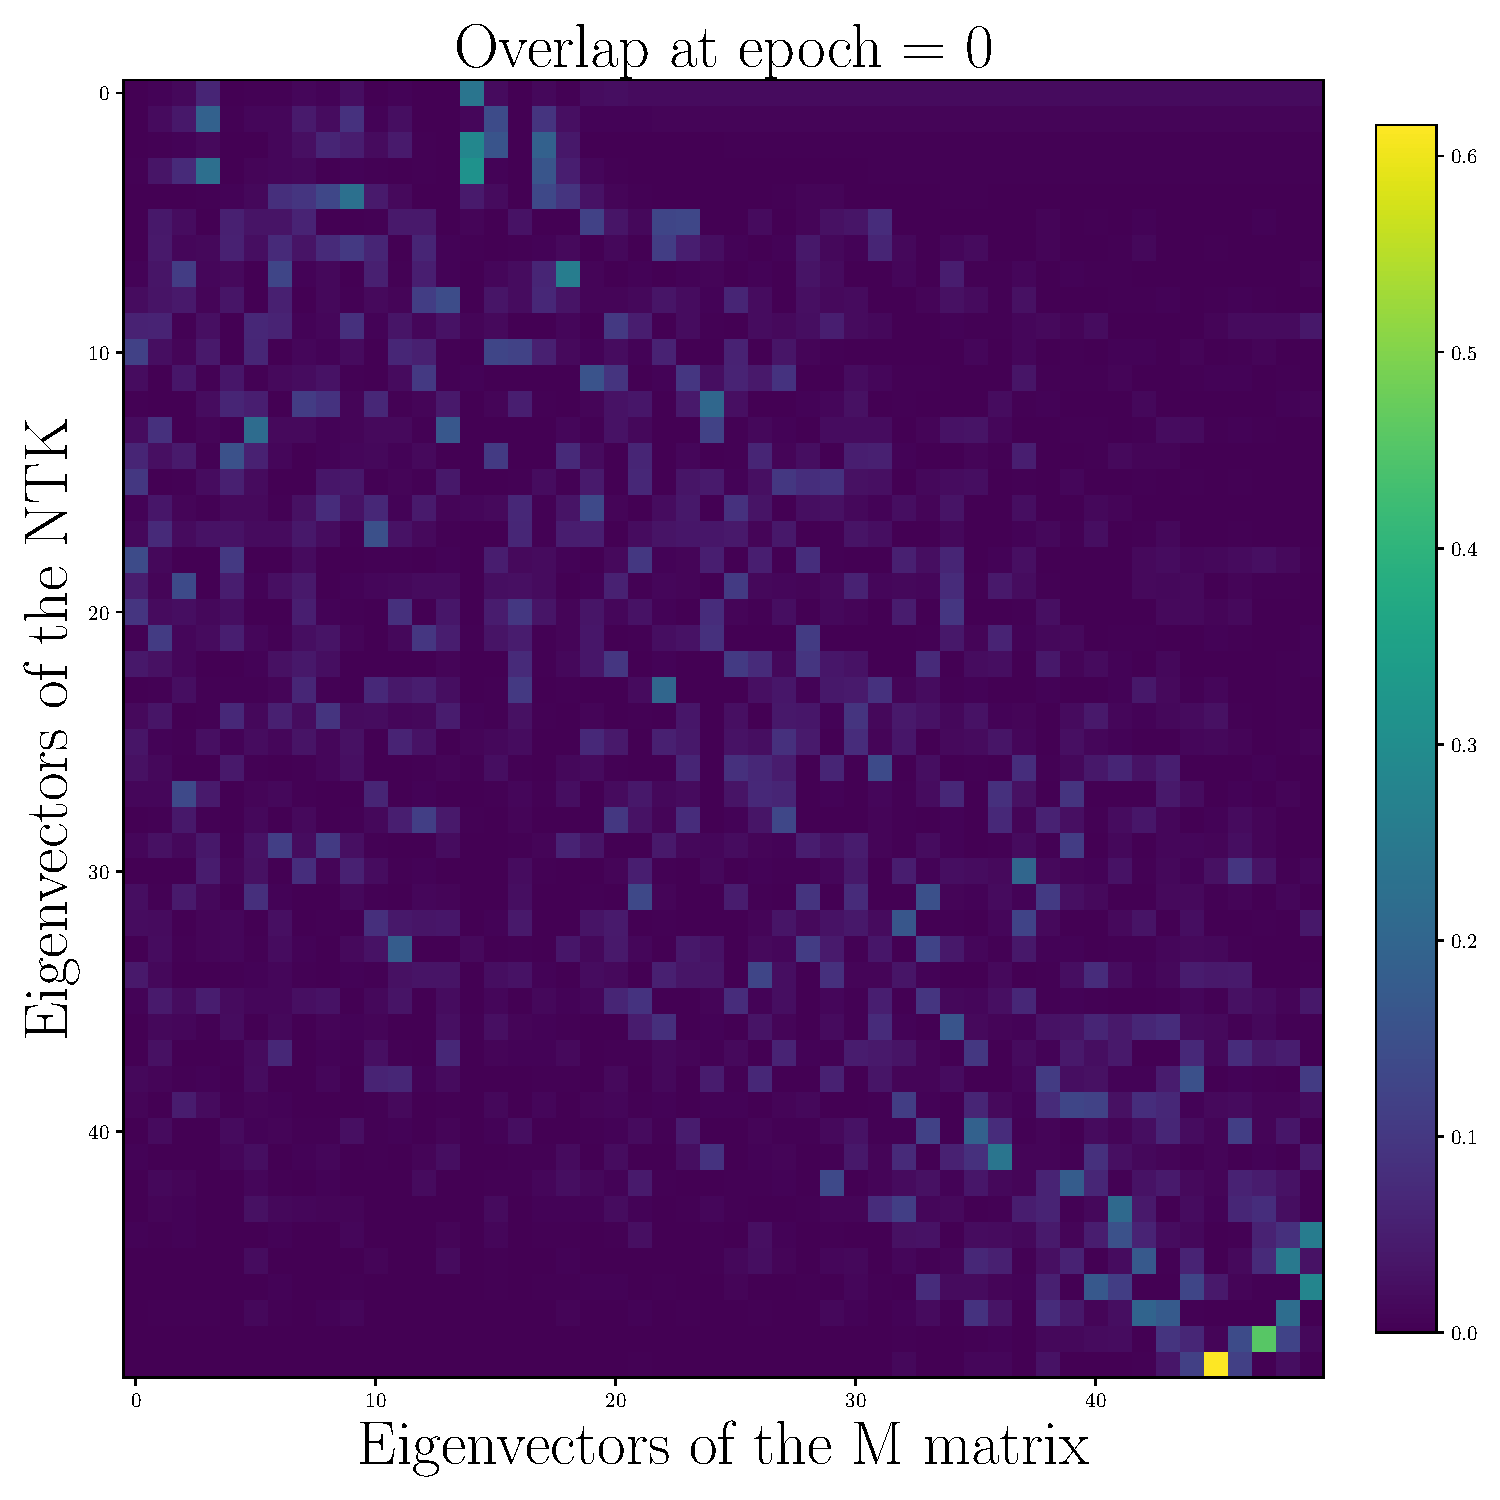
\includegraphics[width=0.45\textwidth]{plots/overlap_epoch_0.pdf}
  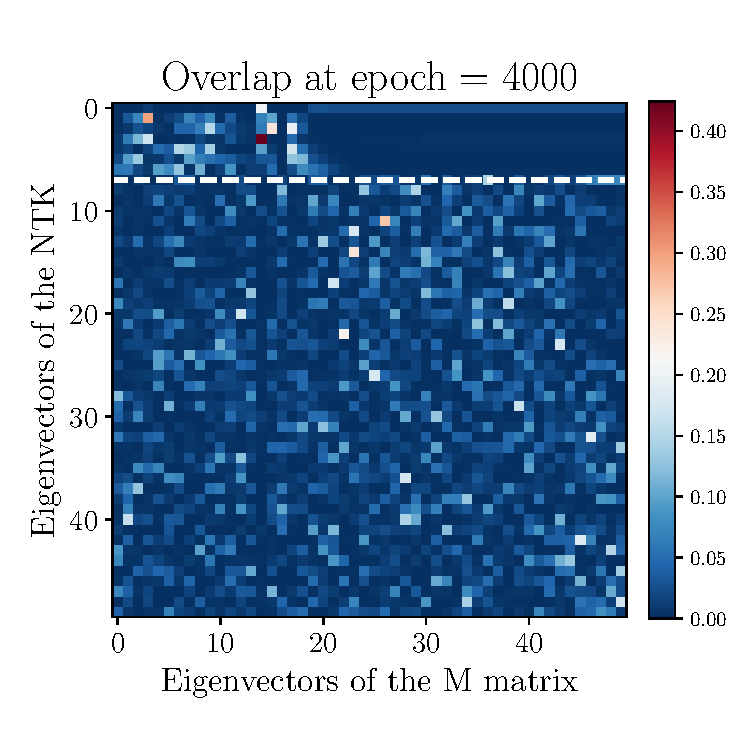
\includegraphics[width=0.45\textwidth]{plots/overlap_epoch_4000.pdf} \\[-15pt]
  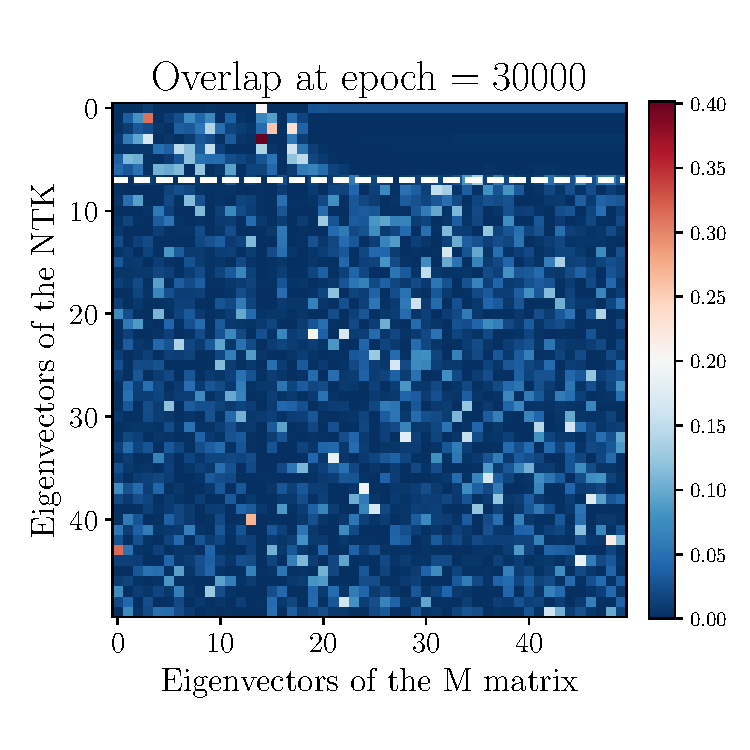
\includegraphics[width=0.45\textwidth]{plots/overlap_epoch_30000.pdf}
  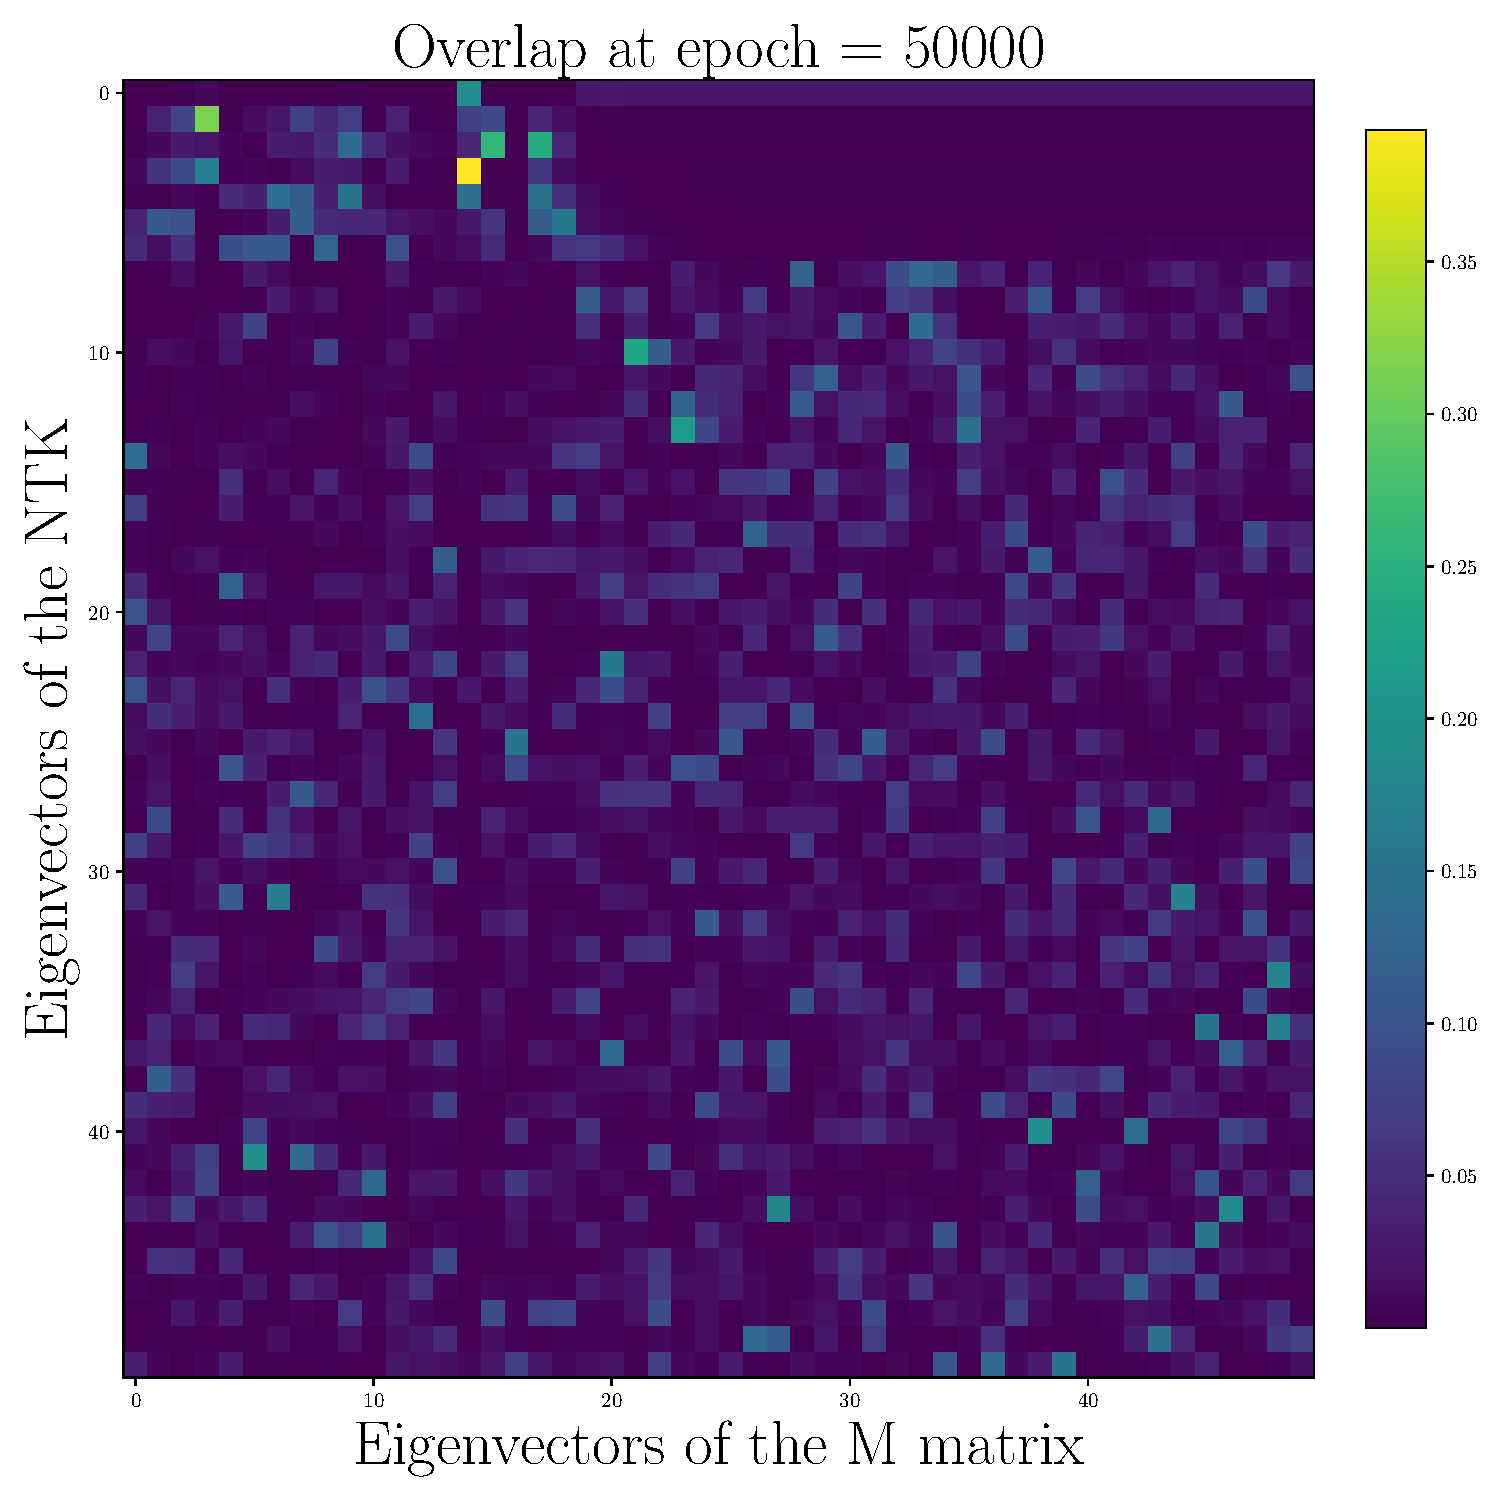
\includegraphics[width=0.45\textwidth]{plots/overlap_epoch_50000.pdf}
  \vspace{0.5cm}
  \caption{Matrix $A$ as defined in Eq.~\eqref{eq:MatrixA} for L1 data and for a single
  replica of the NTK. The matrix is shown at different epochs of the training process,
  indicated in the top of each panel. The white dashed line indicates the cut-off
  tolerance that we imposed to the eigenvalues of the NTK (see Appendix...?).}
  \label{fig:NtkMAlign}
\end{figure}
% ===================================
It has been argued before that there is a non-trivial interplay between the eigenspace of
the NTK and that of the matrix $M$. Indeed, the former encodes the model dependence, while
the latter brings physical information. Of course the two matrices are independent at
initialisation, and we do not expect any alignment patter between the two. However, this picture
might change during training, as the NTK evolves and the model learns the target function.
To quantify this alignment, we define the matrix $A$ as
\begin{equation}
  A_{kk'} = \left( \left< z^{(k)}, v^{(k')}\right> \right)^2 = \cos^2(\theta_{kk'}) \;,
  \label{eq:MatrixA}
\end{equation}
where $z^{(k)}$ and $v^{(k')}$ are the $k$-th and $k'$-th eigenvectors of the NTK and
$M$, respectively. The matrix $A$ is thus a measure of the alignment between the eigenspaces of
the two matrices. In Fig.~\ref{fig:NtkMAlign}, we show the matrix $A$ at different epochs of
the training for L2 data and for a single NTK replica.
